\documentclass[12pt,a4paper]{article}
\usepackage{styles}

\lstset{style=sharpc, tabsize=1}

\renewcommand{\sectionbreak}{\clearpage}

\newcommand{\texta}{Stärken\\[-1ex]}
\newcommand{\textb}{Schwächen\\[-1ex]}
\newcommand{\textcn}{Chancen\\[-1ex]}
\newcommand{\textdn}{Risiken\\[-1ex]}

\author{Alexander van Schie \& Oli Dias}
\title{Gruppenarbeit 3 - Abschliessende Analyse des Providers und Cloud Application Design}
\begin{document}
\maketitle
\newpage
\tableofcontents
\newpage
\section{Analyse Service Level Agreegment (SLA)}
\begin{itemize}
    \item 1. Es wird eine etwas andere Art von SLO’s gemacht, nämlich wird das Problem nach Schwerheitsgrad klassifiziert und je schlimmer es ist, desto schneller muss RedHat reagieren (https://access.redhat.com/support/offerings/openshift/sla)
    \item 2. Openshift gibt in seinem SLA bekannt, dass keine Garantien für Service Uptime besteht. Ebenfalls besteht keine Garantie für Performance. Somit basieren die Service Erbringungen auf gegenseitiges Vertrauen. Dem Kunden werden somit bei jeglichen unzureichenden Serviceleistungen kein Kredit oder Guthaben gewährt.
    \item 3. Generell werden keine Metriken oder Messwerte erwähnt. Vielmehr werden Probleme zusammengefasst und nach Schwerheitsgrad klassifiziert. (https://www.openshift.com/legal/terms/)
    \item 4. Je nach SLA müssen verschieden Dinge eingehalten werden. Was mir persönlich als wichtig erscheint ist eine Vereinbarung bezüglich dem Kundensupport innerhalb einer gewissen Zeit da (a) ein Unterbruch meiner Applikation je nachdem grosse Konsequenzen für mein Unternehmen haben kann. Grundsätzlich sollte ein Cloud-Provider ausgewählt werden, der quasi to big to fail ist (b).
    \item 5. Je nach Branche muss man sich mit den Datenschutzbestimmungen des Cloud Providers auseinander setzen. Beispielsweise wäre es für Banken nicht gerade ideal, Kundendaten auf ausländische Server zu migrieren/verwalten. Generell muss man sich als Kunde eines Cloud Anbieters selbst um die zu treffenden Sicherheitsvorkehrungen bezüglich Daten kümmern.
\end{itemize}

\section{Hands-On Lakeside Mutual}
Die zu deployenden Komponenten lassen sich in zwei Kategorien einteilen; Frontend und Backend. Das Setup der beiden Teile des Backends werden im nachfolgenden Unterkapitel besprochen, das Frontend im Unterkapitel \ref{subsec:frontend}. 

\subsection{Spring Boot Backend Setup}
Für das Migrieren des Backends der Lakeside Mutual DDD Applikation eignet sich für die beiden Komponenten Customer-Core und Customer-Management-Backend ein Wildfly Projekt auf Openshift. Dies sollte analog wie schon beim Deployment der Self-Information Applikation funktionieren, da alle drei Applikationen Spring Boot verwenden. 

Dazu sind folgende Schritte notwendig:
\begin{enumerate}
	\item Hinzufügen der \texttt{.s2i/bin/run} Datei in beiden Spring Boot Apps, die den Befehl für das Ausführen des gebuildeten Jar Files enthält:
	\begin{lstlisting}
	exec java -jar /wildfly/standalone/deployments/
	 customer-management-backend-0.0.1-SNAPSHOT.jar
	\end{lstlisting}
	\item Anpassen der Application-Properties in Customer-Management-Backend: 
	\begin{itemize}
		\item Property \texttt{customercore.baseURL} auf die URL des Customer Cores einstellen. Diese ist gemäss Abbildung \ref{fig:os-routes} in Openshift Cloud herauszufinden. 
		\item Property \texttt{server.port} aus derselben Übersicht auslesen und setzen (Default 8080)
	\end{itemize}
	\item Anpassen der Application-Properties in Customer-Core:
	\begin{itemize}
		\item Property \texttt{server.port} setzen (Default 8080)
	\end{itemize}
\end{enumerate}

\begin{figure}[h]
	\centering
	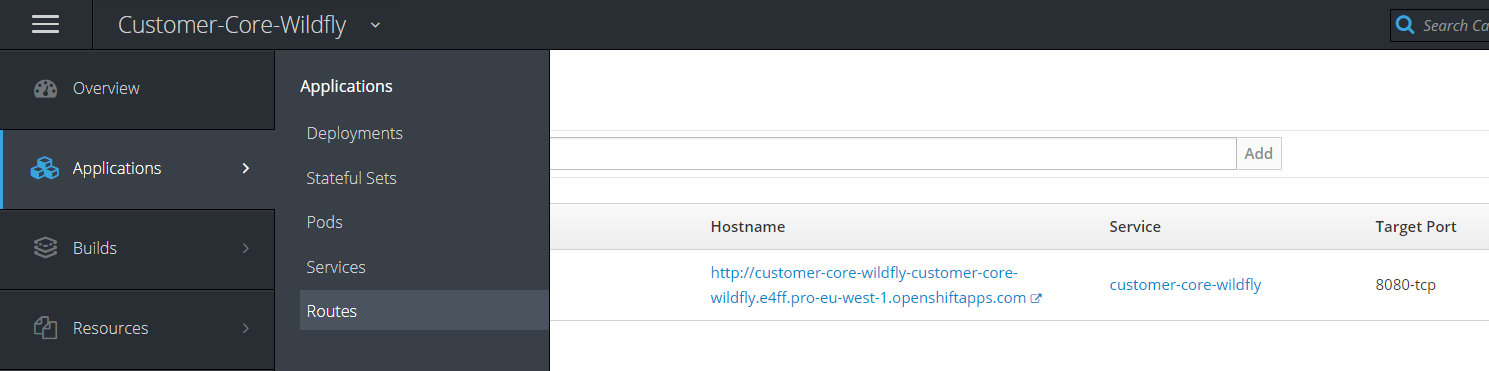
\includegraphics[width=1\linewidth]{img/os-routes}
	\caption{Navigation zu Routes}
	\label{fig:os-routes}
\end{figure}

Da Customer-Management-Backend von der Komponente Customer-Core abhängig ist, muss Customer-Core zuerst deployt werden. Ansonsten wirft die Applikation eine Laufzeit-Exception, da keine Verbindung zum Core hergestellt werden kann. 

Mit dem beschriebenen Setup trafen wir auf eine Hürde: eine \texttt{Request\-Rejected\-Exception}, welche das Ausführen verhinderte. Dazu mehr im Kapitel \ref{subsec:challenges}

\subsection{Frontend Deployment}\label{subsec:frontend}
Openshift bietet Node.js Projekte an, welches sich für die React App eignet. 

Nachdem das Nodejs-Projekt erstellt und das GitHub-Repository erstellt ist, beginnt ein zuständiger Pod gleich mit dem Build. Unglücklicherweise wurde mit unserem Setup an dieser Stelle der Build unterbrochen aufgrund von Limiten, die unsere Subscription setzt. Da das Frontend aber von beiden anderen Komponenten abhängig ist, bleibt uns nichts anderes übrig, als die Frontend-Komponente lokal auszuführen. 

\begin{figure}[h]
	\centering
	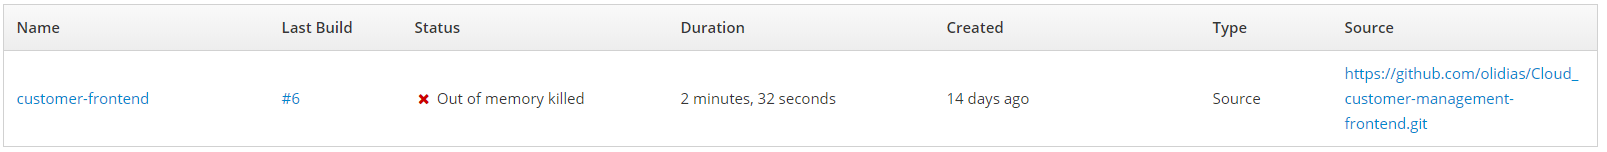
\includegraphics[width=1\linewidth,height=2cm]{img/os-frontend-build-fail}
	\caption{Build-Failure aufgrund von Memory-Limiten}
	\label{fig:os-frontend-build-fail}
\end{figure}

Für die lokale Ausführung wird Node.js benötigt. Ist dies installiert, ist noch eine zusätzliche Konfiguration nötig: Wir müssen auf das Management-Backend zugreifen können und dafür die URL anpassen. Wie im vorgehenden Kapitel schon erwähnt, findet man den URL des Management-Backends in dessen Projekt auf Openshift unter Applications $\rightarrow$ Routes. Die URL muss im File \texttt{src/config.js} angepasst werden:
\begin{lstlisting}[showstringspaces=false]
export const customerManagementBackend =
 getEnvironmentVariable(
  "REACT_APP_CUSTOMER_MANAGEMENT_BACKEND",
  "http://customer-management-backend.e4ff.
    pro-eu-west-1.openshiftapps.com/"
)
\end{lstlisting}
Sind diese Schritte durchgeführt, kann die WebApp mit \texttt{npm start} ausgeführt werden. Es sollte automatisch der Browser mit dem Frontend aufgerufen werden. 

Mit dem erläuterten Setup hat das Frontend wie gewünscht funktioniert, sogar mit dem Chat, dessen History nach einem Neustart immernoch vorhanden war. 

\subsection{Herausforderungen}\label{subsec:challenges}

Es stellte sich beim Deployment dieser drei Komponenten ein grösseres Problem: eine \texttt{RequestRejectedException}, die von Spring-Security entstand. Quelle dieser Exception ist die \texttt{HttpFirewall} von Spring. Diese verhindert, dass URLs mit Doppelslash aufgerufen werden können mit der Begründung, dass solche URLs von Pattern Matching nicht korrekt prozessiert werden könnten oder Pfad-Traversierungen möglich wären \footnote{\url{https://docs.spring.io/spring-security/site/docs/5.0.0.RELEASE/reference/htmlsingle/\#request-matching}}. 

Um dieses Problem zu umgehen, kann ein neues Bean erstellt werden, dass eine \texttt{DefaultHttpFirewall} zurückgibt, die die erläuterte Überprüfung nicht macht. Folgende Methode wurde der Klasse \texttt{Web\-Security\-Configuration.java} hinzugefügt:

\begin{lstlisting}
@Bean
public HttpFirewall allowUrlEncodedSlashHttpFirewall(){
	return new DefaultHttpFirewall();
}
\end{lstlisting}
Durch das Erstellen eines Beans mit Rückgabetyp \texttt{HttpFirewall} verwendet Spring dieses und überschreibt somit das unerwünschte Verhalten. Mit diesem Work-around läuft nun das Customer-Management-Backend wie gewünscht.

\section{Hands-On Persistence}
In diesem Kapitel geht es darum, die bestehende In-Memory-Datenbank mit Mysql zu ersetzen. Zuerst wird das Setup erläutert, nachfolgend die Probleme dargestellt. 

\subsection{Setup}

Für das Persistieren der Kundendaten eignet sich die Openshift Mysql Projekt-Vorlage. Dazu haben wir die Default-Einstellung fürs Erstellen eines solchen Projektes verwendet, bis auf den DB-Namen, den wir auf \texttt{customer\_core} gesetzt haben. 

Um die Spring-Applikationen nun mit dieser Datenbank zu verbinden, müssen wir zuerst den Connection String zusammenbauen. Dazu gibt es folgendes zu beachten: Openshift deployt das Mysql-Image in einem separaten Netzwerk, welches zunächst nicht vom Internet her zugreifbar ist. Es gibt zwei Möglichkeiten, dennoch Zugriff darauf zu bekommen. Entweder die zugreifende Spring Applikation muss in das selbe Netzwerk deployt werden, oder wir müssen zusätzlich eine Route konfigurieren, sodass vom Internet her auf die Datenbank zugegriffen werden kann. 

Wir haben die zweite Möglichkeit ausprobiert und folgende URL herausgefunden:
\begin{lstlisting}
spring.datasource.url = jdbc:mysql://
 persistence-route-customer-core-persistence.e4ff.
 5pro-eu-west-1.openshiftapps.com:3306/customer_core
\end{lstlisting}
Zusätzlich muss noch eine Dependency für den Mysql-Connector in das \texttt{pom.xml} hinzugefügt und den h2 Treiber aus der Konfiguration genommen werden (Zeile mit \texttt{driver\-ClassName} in \texttt{application.properties} auskommentieren). 

Beim Deployment dieser Änderungen zeigten uns die Logdaten eine \texttt{Com\-munications\-Exception}. Nach etwas Recherche fiel auf, dass der Persistence Container ständig eine Fehlermeldung logt:

\begin{figure}[h]
	\centering
	
\includegraphics[width=1\linewidth]{img/os-persistence-error}
	\caption{Fehlermeldung Persistence Container}
	\label{fig:os-persistence-error}
\end{figure}

Die Vermutung ist, dass uns dieser Fehler daran hindert, auf die Datenbank in der Cloud zuzugreifen. 
 
Im Umfang dieses Assessment konnte die Ursache dieses Problems nicht gefunden werden, aber im folgenden Kapitel werden die getroffenen Massnahmen dargestellt.

\subsection{Herausforderungen}
Für die Fehlerbehandlung des in \ref{fig:os-persistence-error} dargestellten Fehlers schlagen einige Entwickler online vor, den Wert der Mysql-Umgebungsvariable \texttt{max\_allowed\_packet} zu erhöhen. Dies wurde durch verschiedene Ansätze probiert, der funktionierende Weg wurde aber in der Openshift-Dokumentation gefunden.  \footnote{\url{https://docs.openshift.com/container-platform/3.3/using\_images/db\_images/mysql.html\#mysql-environment-variables}}
Der Wert dieser Variable (und Umgebungsvariablen allgemein) kann in der Openshift Console unter Applications $\rightarrow$ Deployments $\rightarrow$ Environment gesetzt werden. Mit dem Kommandozeilentool \texttt{oc} kann weiter auf die Mysql Instanz per remote Shell zugegriffen werden und die Umgebungsvariablen mittels 
\begin{lstlisting}
show variables;
\end{lstlisting}
abgefragt werden. Die Updates können so beobachtet werden, jedoch scheint dies keine Wirkung auf das Problem zu haben. Es werden auch dann noch im 10-Sekunden-Takt diese Logmeldungen ausgegeben. 

Diese generische Fehlermeldung machte es uns schwierig, das genaue Problem zu entdecken und konnten es deshalb nicht beheben.



\section{Twelve-Factor Apps - Engineering Projekt}
    \begin{table}[H]
        \begin{tabular}{ll}
        \hline
        \textbf{Erfüllt}      & \textbf{Nicht erfüllt}     \\ \hline
        Codebase              & Dev/prod parity            \\ \hline
        Dependencies          & Logs                       \\
        Config                &                            \\
        Backing services      &                            \\
        Build, release, run   &                            \\
        Processes             &                            \\
        Port binding          &                            \\
        Concurrency           &                            \\
        Port binding          &                            \\
        Disposability         &                            \\
        Admin processes       &                            \\ \hline
        \end{tabular}
    \end{table}

\subsection{Anpassungen}
    \begin{itemize}
        \item Dev/prod parity: Die ganze Applikation wurde nur auf einem System entwickelt. Sobald Code eingecheckt und die Tests
              erfolgreich waren, war der Code bereits produktiv. Die Anpassung lautete somit mehrere Umgebungen gleichzeitig zu
              unterhalten.
        \item Logs: Das Verhalten der Applikation wurde mit Enduser-Tests überprüft. Die Anpasssung beinhaltet somit die Erfassung
              von Logs bei der Interaktion mit unserer Applikation.
    \end{itemize}

\subsection{Unterschied zu IDEAL Architektur}

Die Twelve-Factor Apps Methode gibt dem Leser konkrete Konzepte, wie gewissen Dinge umgesetzt werden sollen. Die IDEAL Cloud Application
Properties hingegen sind auf einer höheren Ebene angesiedelt und geben mehr vor, mit welchen Patterns die jeweilige Eigenschaft erfüllt werden kann.
Somit werden die 12 Schritte bereits mit einem Pattern, welches von IDEAL vorgeschlagen wird, umgesetzt. Wie auch in den Vorlesungsfolien zu entnhemen ist,
sind die 12 Schritte im Einklang mit IDEAL.

\subsection{Fazit}
Abschliessend lässt sich die Twelve-Factor Apps Methode einfacher realisieren, da die Schritte als Checkliste verwendet werden können.
Hierzu sind die IDEAL-Properties auf einem zu hohen Level definiert.

\section{Security Features und Assessment}

In den Terms und Conditions von Openshift ist ganz klar zu entnehmen, dass der Anwedender für Themen des Datenschutzes die Verantwortung übernimmt.
So hat der Anwender sicherzustellen, dass die Daten der Anwender seiner Applikation geschützt werden. Dies beinhaltet die Implementation von
Datnschutzrichtlinien, welche rechtlich abgestimmt sind. Zudem müssen die Anwender darüber informiert werden, dass ihre Daten auf der Infrstruktur
von Red Hat abgelegt wird und sie dem somit zustimmen.

Red Hat gibt bekannt, dass folgende Technologien von ihrem PaaS unterstützt werden:

\begin{itemize}
    \item SELinux
    \item Process, network, and storage separation
    \item Stateful and stateless inspection firewall
    \item Proactive monitoring of capacity limits
    \item Intrusion detection
    \item Port monitoring
    \item Pam namespace
    \item Security compliance frameworks
    \item RPM verification and vulnerabilities updated
    \item Remote logging
    \item Encrypted communications
\end{itemize}
https://www.openshift.com/policy/security/

\subsection{Checkliste Security Assessment}


\begin{table}[H]
    \begin{tabular}{lr}
    \hline
    \textbf{Anforderung}                   & \textbf{Erfüllungsgrad} \\ \hline
    1. Encrypted Communication             & 10                      \\
    2. Backups                             & 3                       \\
    3. Location                            & 7                       \\
    4. Server Redundancy                   & 8                       \\
    5. Service Authentification            & 10                      \\
    6. Appropriate SLA                     & 7                       \\
    7. Data Isolation                      & 10                      \\
    8. Transparency (Monitoring)           & 8                       \\
    9. Network Design und Logging          & 6                       \\ \hline
    \end{tabular}
\end{table}

\subsubsection{Bemerkungen}

1. Openshift nutzt Kubernetes und die Kommunikation bei Kubernetes ist standardmässig mit TLS verschlüsselt.

2. Backups müssen selbst gemacht werden, es gibt hierfür keinen Service. Positive ist jedoch, dass das Vorgehen dokumentiert ist.

3. Openshift wird vermutlich Data Centers an mehreren geographischen Standorten haben, kommuniziert dies jedoch nicht öffentlich.

4. Da Openshift mit Kubernetes arbeitet, besteht auch die Möglichkeit der Nutzung von Replicas, diese müssen jedoch selbst definiert werden.

5. Authentifizierungserfahren laufen über OAuth und bietet alle gängigen Möglichkeiten (\url{https://docs.openshift.com/enterprise/3.0/admin_guide/configuring_authentication.html})

6. Es gibt ein SLA, in dem wichtige Punkte zur Einhaltung der Servicebedingungen festgehalten sind. Was jedoch nicht zu entnehmen ist, sind Strafen, die bei Nichteinhaltung fällig werden.

7. Kubernetes NetworkPolicy wird voll unterstützt und Projekte können ebenfalls in einer isolierten Umgebung betrieben werden.

8. Quotas sowie laufende Prozesse können eingesehen werden

9. Standardmässig werden Logs geschrieben, diese waren unserer Erfahrungen nach unzureichend (was das Fehlerhandling erschwerte)

\section{SWOT-Assessment von Cloud Provider und Cloud Offering}

\begin{tikzpicture}[font=\small,
        any/.style={draw, text width=.5\linewidth-1cm, align=center,               anchor=center, inner sep=5pt},
        row 1/.style={nodes={any, minimum height=1cm, fill=black!10}},
        row 2/.style={nodes={any, minimum height=9cm}},
        row 3/.style={nodes={any, minimum height=8cm}},
        row 2 column 1/.style={nodes={any, minimum height=1cm, fill=black!10, rotate=90, minimum width=9cm}},
        row 3 column 1/.style={nodes={any, minimum height=1cm, fill=black!10, rotate=90, minimum width=8cm}}
    ]
    \matrix (SWOT) [matrix of nodes, inner sep=0pt,
    column sep=-1\pgflinewidth,
    row sep=-1\pgflinewidth,
    inner sep=0pt]
    {
     & {\texta} & {\textb} \\
     {\textcn} & \begin{itemize}
        \item Web App Design
        \item Einfache Projektinitialisierung
        \item Command Line Interface (CLI)
    \end{itemize} &\begin{itemize}
        \item Limitierte Ressourcen
        \item Limitierete Projektauswahl
        \item Limitierte Abonnemente
        \item Preis
        \item Fehlende Service Garantie
    \end{itemize} \\
     {\textdn} & \begin{itemize}
        \item Nutzung von Kubernetes
        \item Ausbaubare Service Dokumentation
        \item Chance zur Änderung (Nicht to big to change)
    \end{itemize} & \begin{itemize}
        \item Transparenz Fehlerbehandlung
        \item Transparenz Nutzungsbedingungen
        \item Ablehnung jeglicher Sicherheitsaspekte
        \item Kleine Community
    \end{itemize} \\
    };
    \draw[fill=black!10] ($(SWOT-1-2.north west)+(\pgflinewidth/2,-\pgflinewidth/2)$) rectangle ($(SWOT-1-3.north east)+(-\pgflinewidth/2,-\pgflinewidth/2+1cm)$)
        node[midway] {Interne Analyse};
    \draw[fill=black!10] ($(SWOT-3-1.north west)+(-1cm+\pgflinewidth/2,\pgflinewidth/2)$) rectangle ($(SWOT-2-1.north east)+(\pgflinewidth/2, -\pgflinewidth/2)$)
        node[midway, rotate=90] {Externe Analyse};
    \end{tikzpicture}

\section{Provider Evaluation Checkliste}
    \begin{table}[H]
        \begin{tabular}{lll}
            \hline
            \textbf{Kriterium}  & \textbf{Erfüllt}                    \\ \hline
            1. Umfangreicher Technologiekatalog     & Jein            \\
            2. Unternehmungsgrösse des Anbieters    & Nein            \\
            3. Customizing                          & Jein            \\
            4. Dokumentation                        & Ja              \\
            5. Community                            & Nein            \\
            6. Support                              & Ja              \\
            7. OSSM                                 & Ja              \\
            8. Globale Data Center                  & Jein            \\
            9. Preis                                & Nein            \\
            10. Usability                           & Ja              \\ \hline
        \end{tabular}
    \end{table}

\subsection{Kommentare}

1. Welches Angebot stellt uns der Anbieter zur Verfügung.

2. Grosse Unternehmen haben tendenziel mehr Erfahrung als Cloud Anbieter.

3. Bedingt durch das Angebot PaaS ist customizing nur bedingt möglich.

4. Eine ausführliche Dokumentation zu den Funktionalitäten ist hier zu finden: \url{https://docs.openshift.com/container-platform/3.11/welcome/index.html}

5. Obwohl die Openshift Community ständig wächst, wird man bei spezifischen Problemen in der Community nicht fündig

6. Wird angeboten. Je nach Abonnement ändert sich die Antwortzeit bei Incidents.

7. Bereits im ersten Teil besprochen.

8. Zwar besitzt Openshift rund um den Globus Data Center, je nach Applikation und Standort gibt es hierbei jedoch bessere Alternativen.

9. Openshift eignet sich (aus preislicher Perspektive) für den Unterhalt von grösseren Applikationen, welche ressourcenlastig sind.

10. Unserer Ansicht nach war das Arbeiten mit der Webkonsole sehr angenehm.

\section{Management Summary}

Openshift bietet eine gute Möglichkeit, kleinere Container basierte Applikationen in die Cloud zu bringen. Aus der Sicht des Entwicklers
ist es ratsam, bereits einige Erfahrungen mit Cloudprojekten gemacht zu haben. Zudem ist ein Basiswissen bezüglich Kubernetes gefordert.
Generell ist es zu empfehlen, bereits im Vorhinein die Kompatibilität der Applikation in der Openshift Container Plattform zu prüfen.
Anderst als bei den grossen Cloud Anbietern hält sich die Community klein und bei einer sehr spezifischen Applikation wird der Deploymentprozess
erheblich erschwert. Als Kunde muss man sich zudem bewusst sein, dass Openshift keinerlei Garantie für die Erbringung der Uptime gewährleistet.
Ebenfalls werden Anträge bezüglich unzureichender Performance seitens Openshift abgelehnt.


Zusammenfassend erweist sich Openshift interessant für Projekte, welche einen gewissen Risikospielraum zulassen. Bei grösseren Applikationen oder
Zeit-/Sicherheitskritischen Applikationen empfiehlt sich eine direkte Kontaktaufnahme mit Openshift, um Unklarheiten zu klären.
    

\end{document}